\documentclass{article}
\usepackage{amsmath}
\usepackage{amsfonts}
\usepackage{amssymb}
\usepackage{multicol}
\usepackage{graphicx}
\usepackage{lipsum}
\usepackage{float}
\title{SteamLineBreak}
\author{Jakub Matl}
\date{\today}
\begin{document}
\maketitle
\begin{multicols}{2}
\begin{figure}[H]
\centering
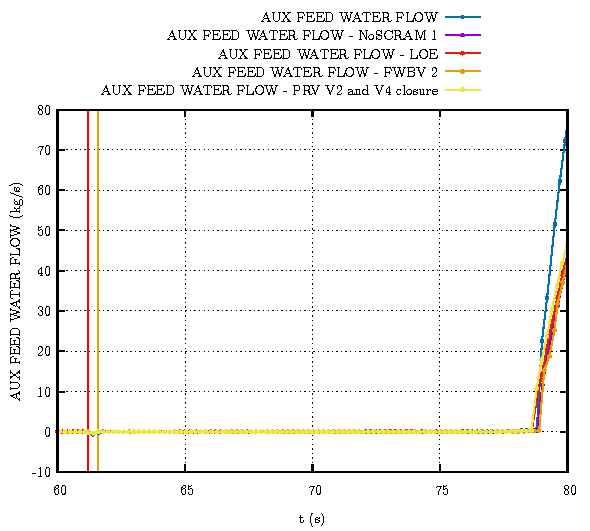
\includegraphics[width=\linewidth]{./graphs/AUX FEED WATER FLOW.pdf}
\end{figure}
\begin{figure}[H]
\centering
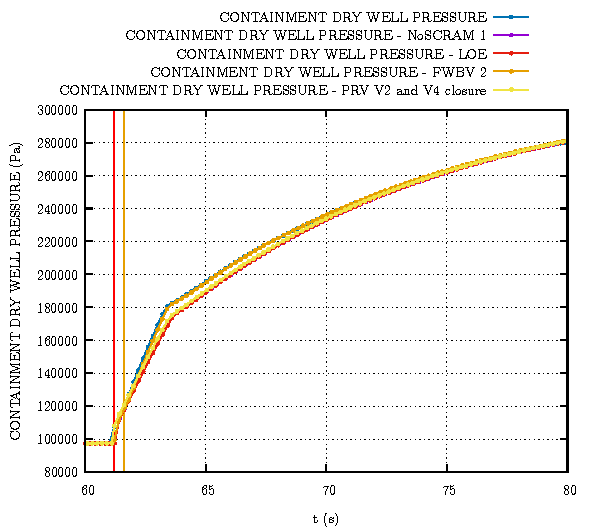
\includegraphics[width=\linewidth]{./graphs/CONTAINMENT DRY WELL PRESSURE.pdf}
\end{figure}
\begin{figure}[H]
\centering
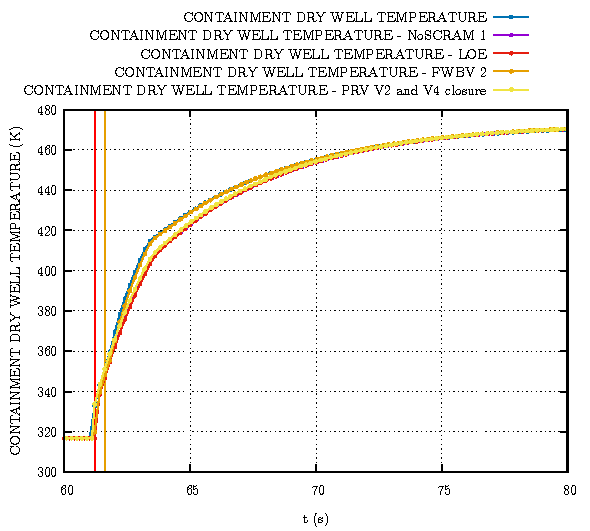
\includegraphics[width=\linewidth]{./graphs/CONTAINMENT DRY WELL TEMPERATURE.pdf}
\end{figure}
\begin{figure}[H]
\centering
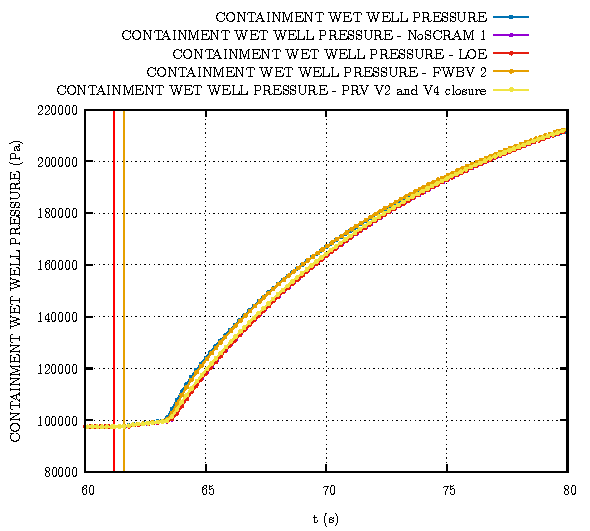
\includegraphics[width=\linewidth]{./graphs/CONTAINMENT WET WELL PRESSURE.pdf}
\end{figure}
\begin{figure}[H]
\centering
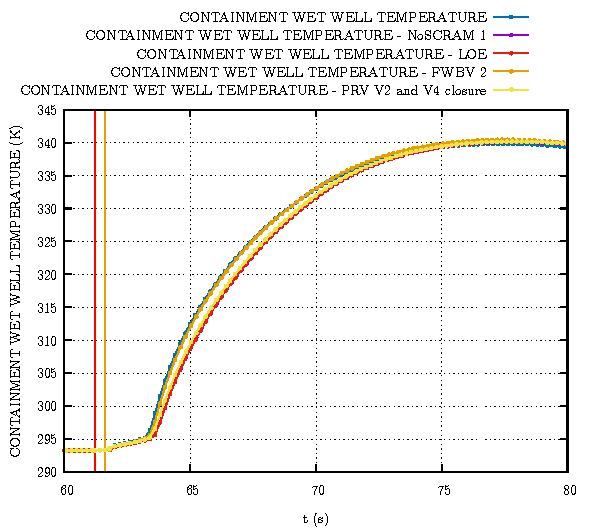
\includegraphics[width=\linewidth]{./graphs/CONTAINMENT WET WELL TEMPERATURE.pdf}
\end{figure}
\begin{figure}[H]
\centering
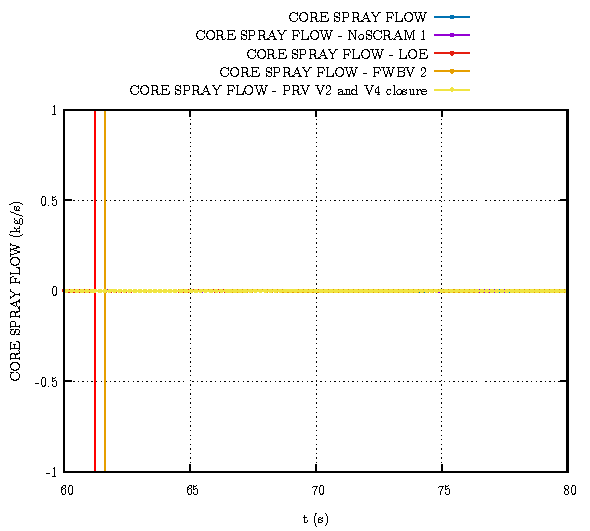
\includegraphics[width=\linewidth]{./graphs/CORE SPRAY FLOW.pdf}
\end{figure}
\begin{figure}[H]
\centering
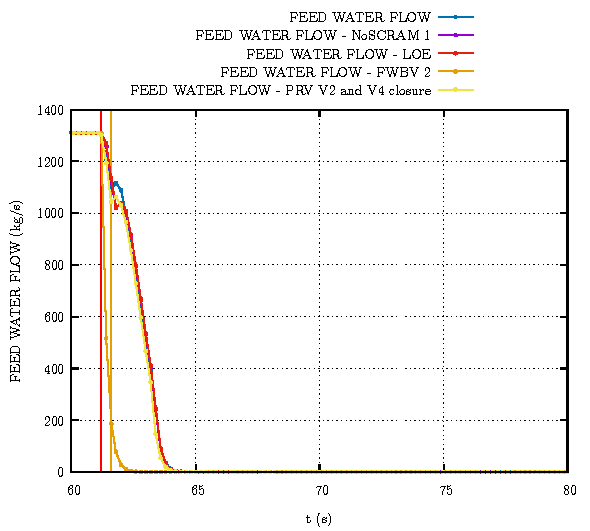
\includegraphics[width=\linewidth]{./graphs/FEED WATER FLOW.pdf}
\end{figure}
\begin{figure}[H]
\centering
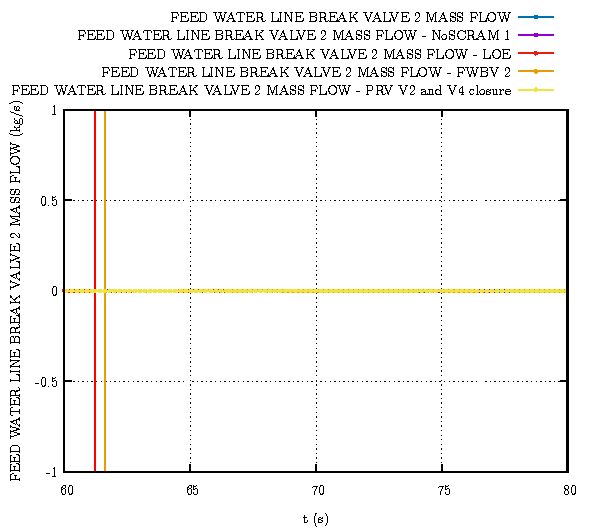
\includegraphics[width=\linewidth]{./graphs/FEED WATER LINE BREAK VALVE 2 MASS FLOW.pdf}
\end{figure}
\begin{figure}[H]
\centering
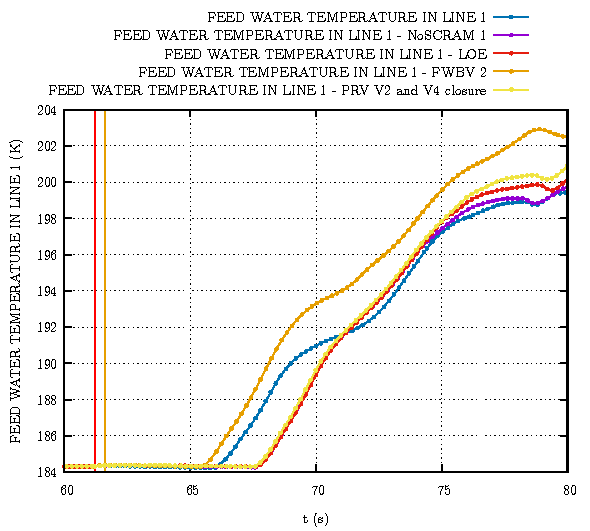
\includegraphics[width=\linewidth]{./graphs/FEED WATER TEMPERATURE IN LINE 1.pdf}
\end{figure}
\begin{figure}[H]
\centering
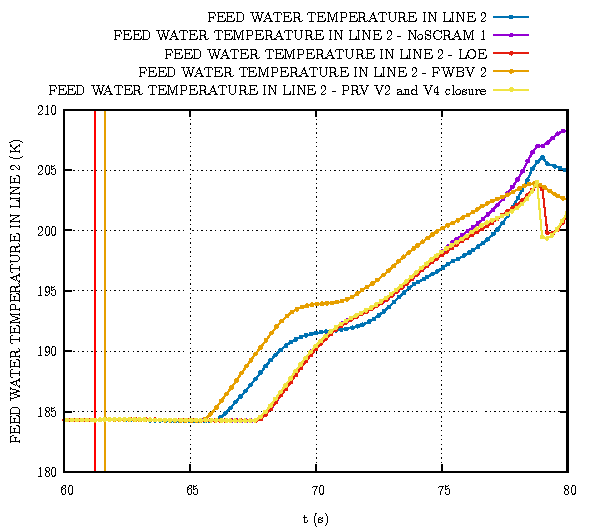
\includegraphics[width=\linewidth]{./graphs/FEED WATER TEMPERATURE IN LINE 2.pdf}
\end{figure}
\begin{figure}[H]
\centering
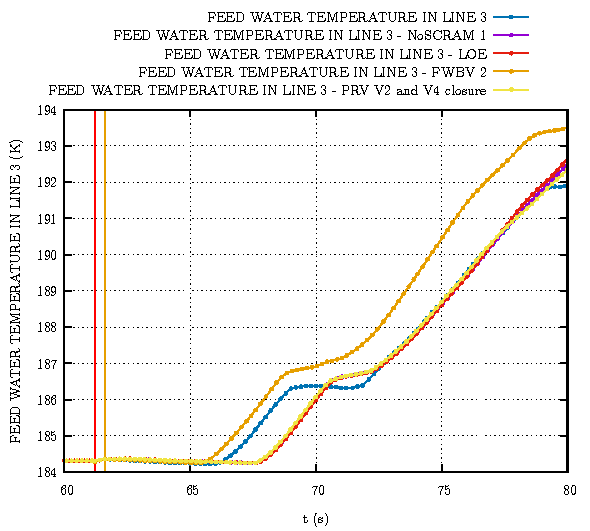
\includegraphics[width=\linewidth]{./graphs/FEED WATER TEMPERATURE IN LINE 3.pdf}
\end{figure}
\begin{figure}[H]
\centering
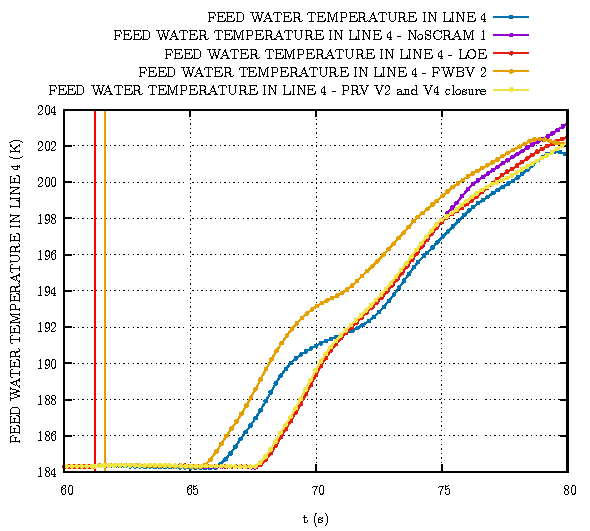
\includegraphics[width=\linewidth]{./graphs/FEED WATER TEMPERATURE IN LINE 4.pdf}
\end{figure}
\begin{figure}[H]
\centering
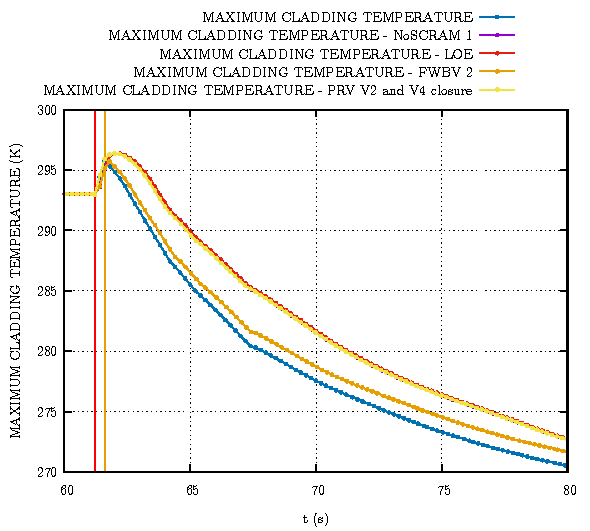
\includegraphics[width=\linewidth]{./graphs/MAXIMUM CLADDING TEMPERATURE.pdf}
\end{figure}
\begin{figure}[H]
\centering
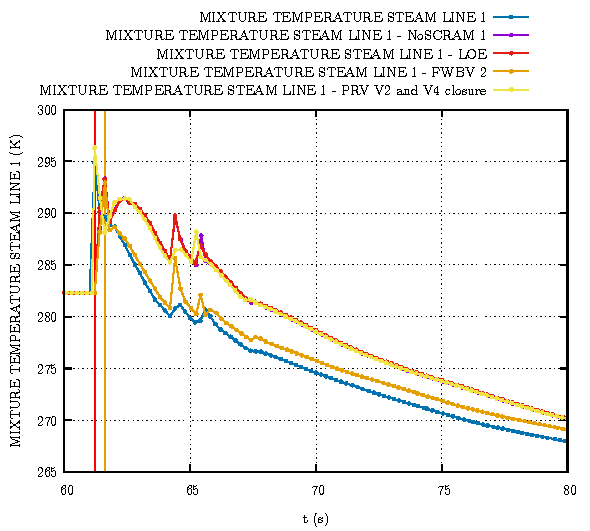
\includegraphics[width=\linewidth]{./graphs/MIXTURE TEMPERATURE STEAM LINE 1.pdf}
\end{figure}
\begin{figure}[H]
\centering
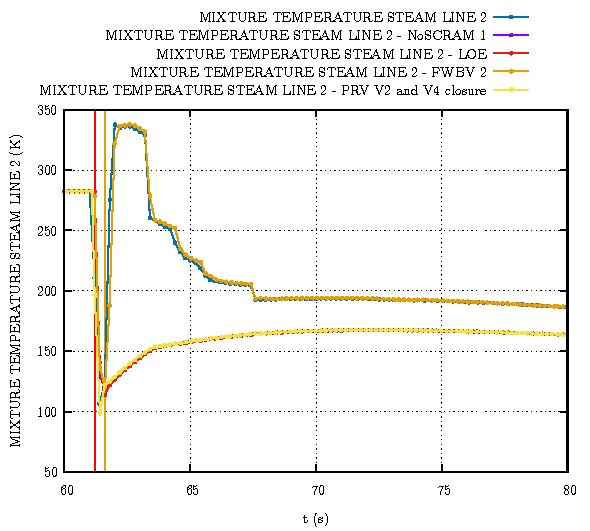
\includegraphics[width=\linewidth]{./graphs/MIXTURE TEMPERATURE STEAM LINE 2.pdf}
\end{figure}
\begin{figure}[H]
\centering
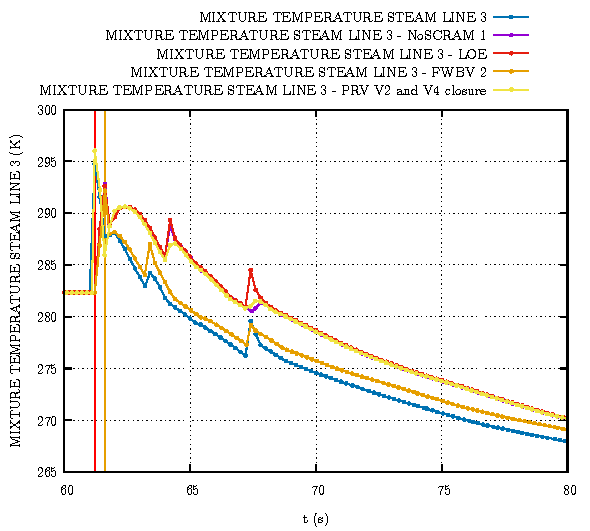
\includegraphics[width=\linewidth]{./graphs/MIXTURE TEMPERATURE STEAM LINE 3.pdf}
\end{figure}
\begin{figure}[H]
\centering
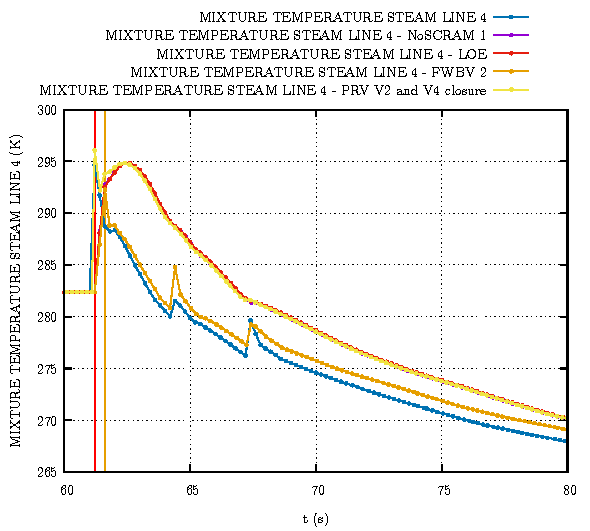
\includegraphics[width=\linewidth]{./graphs/MIXTURE TEMPERATURE STEAM LINE 4.pdf}
\end{figure}
\begin{figure}[H]
\centering
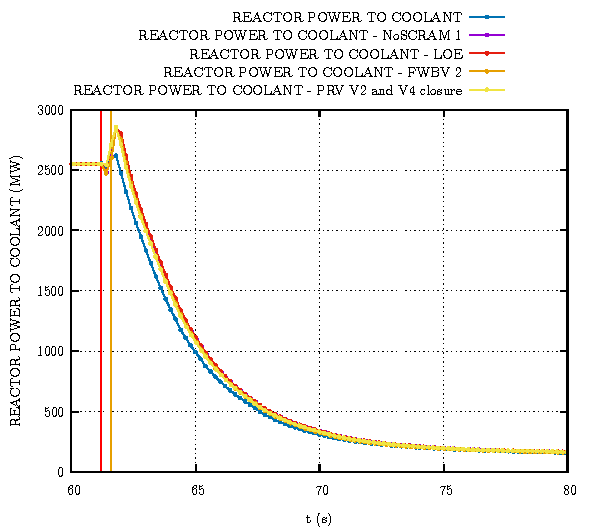
\includegraphics[width=\linewidth]{./graphs/REACTOR POWER TO COOLANT.pdf}
\end{figure}
\begin{figure}[H]
\centering
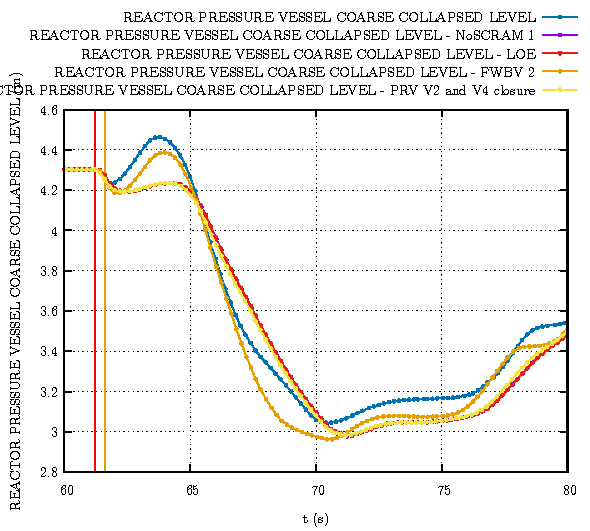
\includegraphics[width=\linewidth]{./graphs/REACTOR PRESSURE VESSEL COARSE COLLAPSED LEVEL.pdf}
\end{figure}
\begin{figure}[H]
\centering
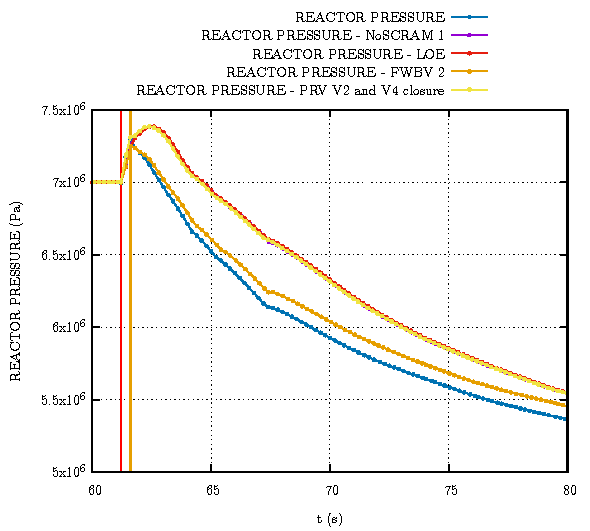
\includegraphics[width=\linewidth]{./graphs/REACTOR PRESSURE.pdf}
\end{figure}
\begin{figure}[H]
\centering
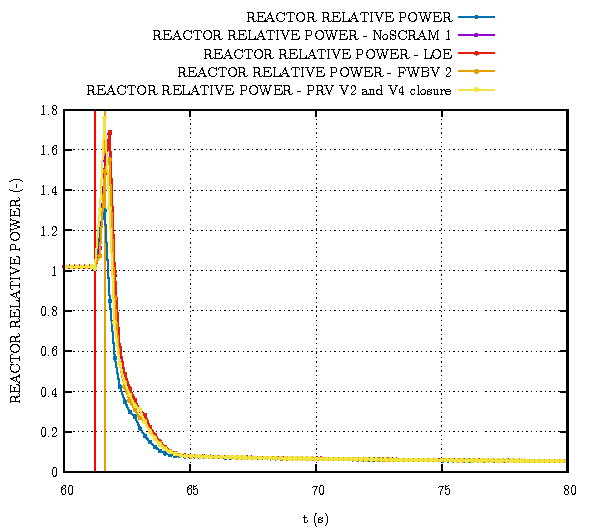
\includegraphics[width=\linewidth]{./graphs/REACTOR RELATIVE POWER.pdf}
\end{figure}
\begin{figure}[H]
\centering
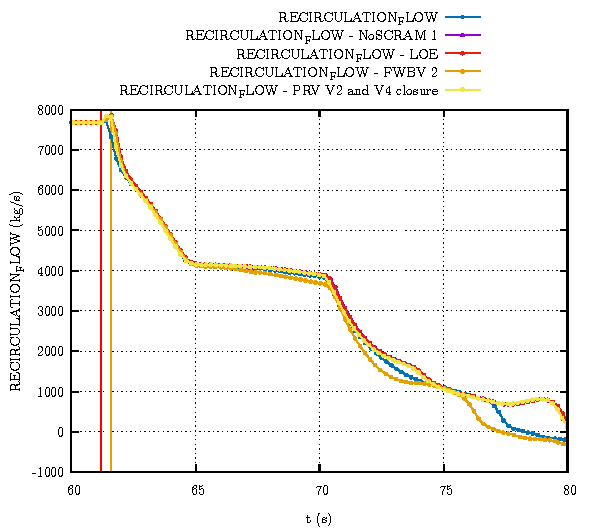
\includegraphics[width=\linewidth]{./graphs/RECIRCULATION_FLOW.pdf}
\end{figure}
\begin{figure}[H]
\centering
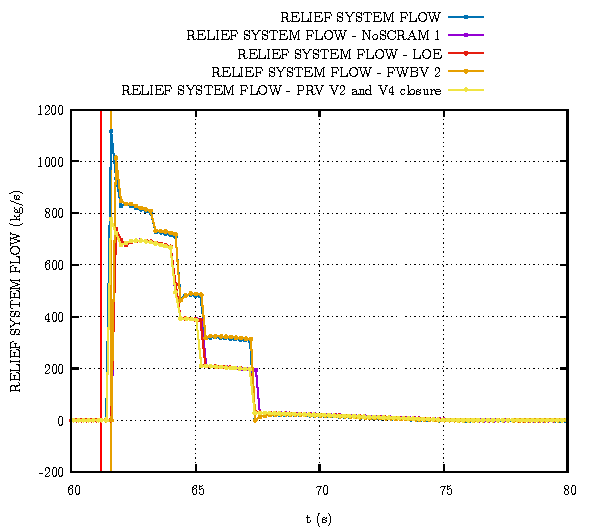
\includegraphics[width=\linewidth]{./graphs/RELIEF SYSTEM FLOW.pdf}
\end{figure}
\begin{figure}[H]
\centering
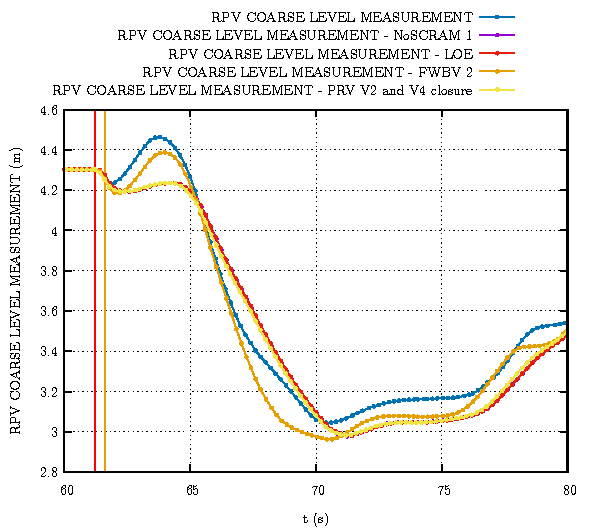
\includegraphics[width=\linewidth]{./graphs/RPV COARSE LEVEL MEASUREMENT.pdf}
\end{figure}
\begin{figure}[H]
\centering
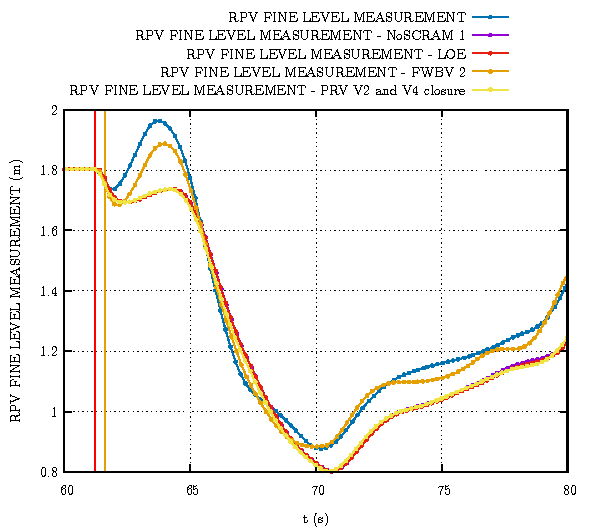
\includegraphics[width=\linewidth]{./graphs/RPV FINE LEVEL MEASUREMENT.pdf}
\end{figure}
\begin{figure}[H]
\centering
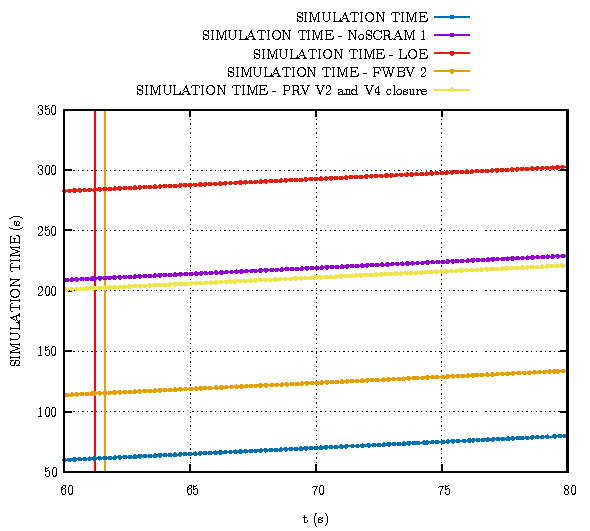
\includegraphics[width=\linewidth]{./graphs/SIMULATION TIME.pdf}
\end{figure}
\begin{figure}[H]
\centering
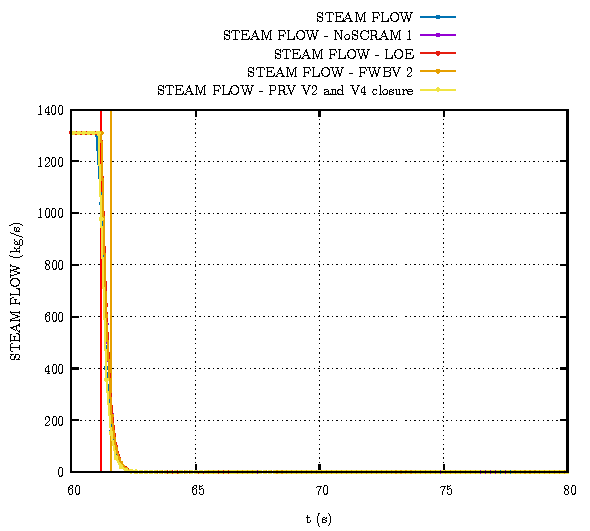
\includegraphics[width=\linewidth]{./graphs/STEAM FLOW.pdf}
\end{figure}
\begin{figure}[H]
\centering
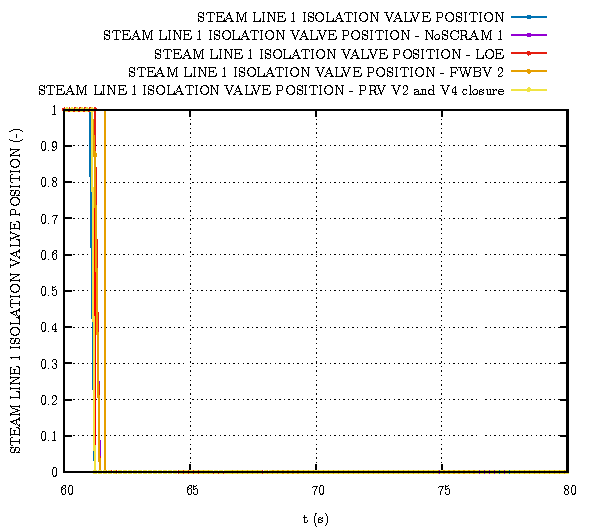
\includegraphics[width=\linewidth]{./graphs/STEAM LINE 1 ISOLATION VALVE POSITION.pdf}
\end{figure}
\begin{figure}[H]
\centering
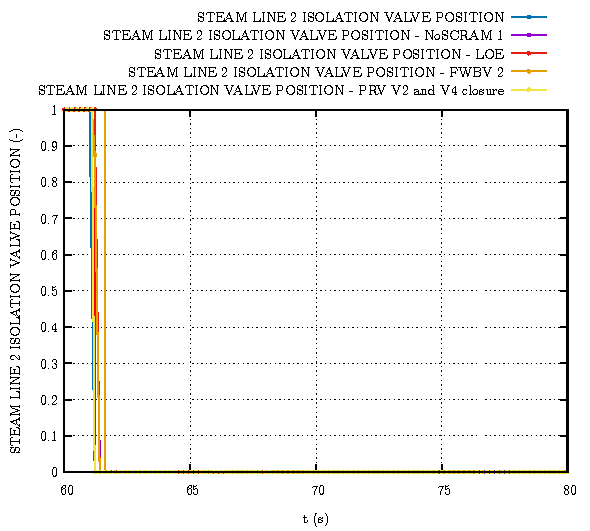
\includegraphics[width=\linewidth]{./graphs/STEAM LINE 2 ISOLATION VALVE POSITION.pdf}
\end{figure}
\begin{figure}[H]
\centering
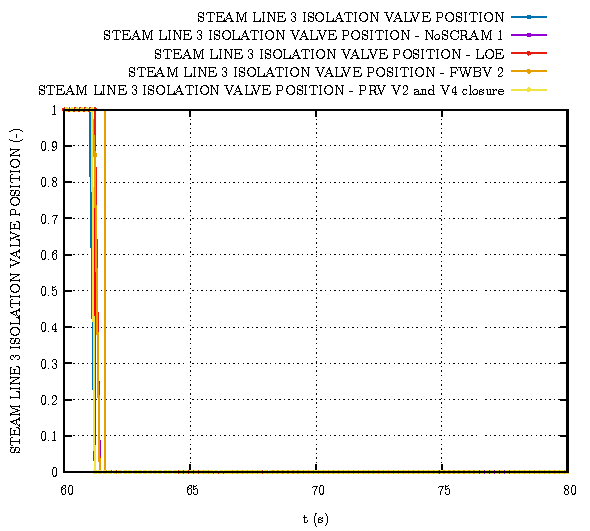
\includegraphics[width=\linewidth]{./graphs/STEAM LINE 3 ISOLATION VALVE POSITION.pdf}
\end{figure}
\begin{figure}[H]
\centering
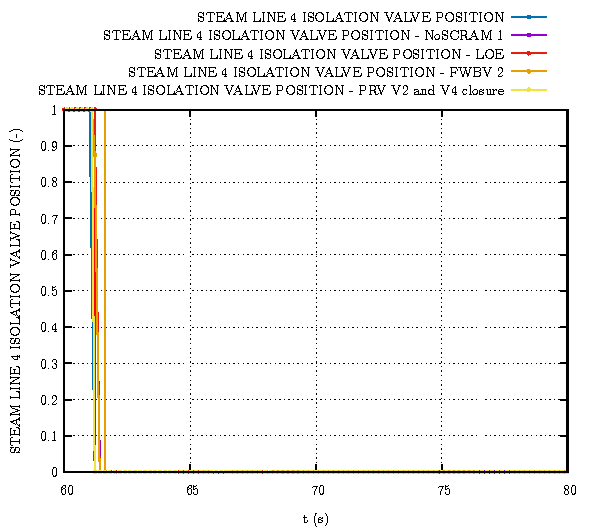
\includegraphics[width=\linewidth]{./graphs/STEAM LINE 4 ISOLATION VALVE POSITION.pdf}
\end{figure}
\begin{figure}[H]
\centering
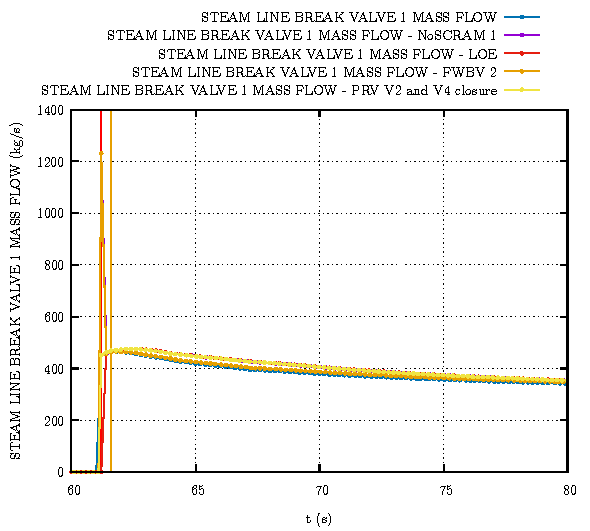
\includegraphics[width=\linewidth]{./graphs/STEAM LINE BREAK VALVE 1 MASS FLOW.pdf}
\end{figure}
\begin{figure}[H]
\centering
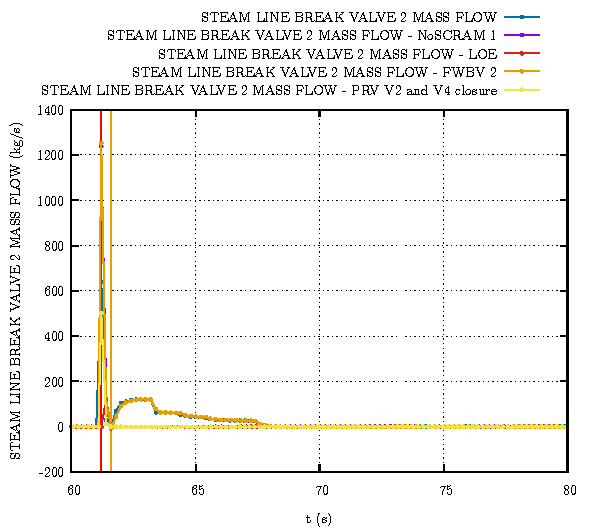
\includegraphics[width=\linewidth]{./graphs/STEAM LINE BREAK VALVE 2 MASS FLOW.pdf}
\end{figure}
\begin{figure}[H]
\centering
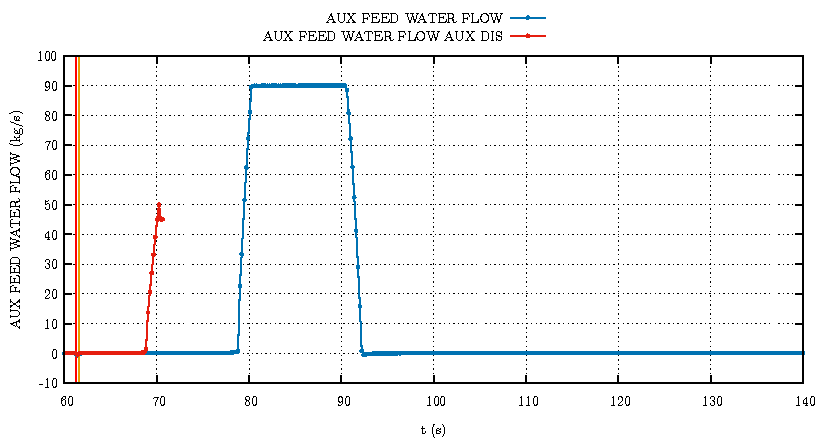
\includegraphics[width=\linewidth]{./graphs/merged.pdf}
\end{figure}
\end{multicols}
\end{document}
